\documentclass[11pt]{article}
%\usepackage{algorithm2e}
\usepackage[utf8]{inputenc}
\usepackage{amsfonts}
%\usepackage{braket}
% \usepackage[bottom]{footmisc}
\usepackage{xcolor}
\usepackage{amsmath}
\usepackage{enumerate}
% \usepackage{appendix}
\usepackage{hyperref}
\usepackage{amsthm}
\usepackage{multirow}
\usepackage{tikz}
\usetikzlibrary{matrix,decorations.pathreplacing,quantikz}
% \usepackage{mleftright}
\usepackage{amssymb}
\usepackage{algorithm}
\usepackage{algpseudocode}
\algrenewcommand\algorithmicrequire{\textbf{Input:}}
\algrenewcommand\algorithmicensure{\textbf{Output:}}
% \usepackage{mathabx}
% \usepackage{comment}
\usepackage{subcaption}
\usepackage{enumerate}
\usepackage[margin=20pt]{geometry}

\usetikzlibrary{math} %needed tikz library

\begin{document}




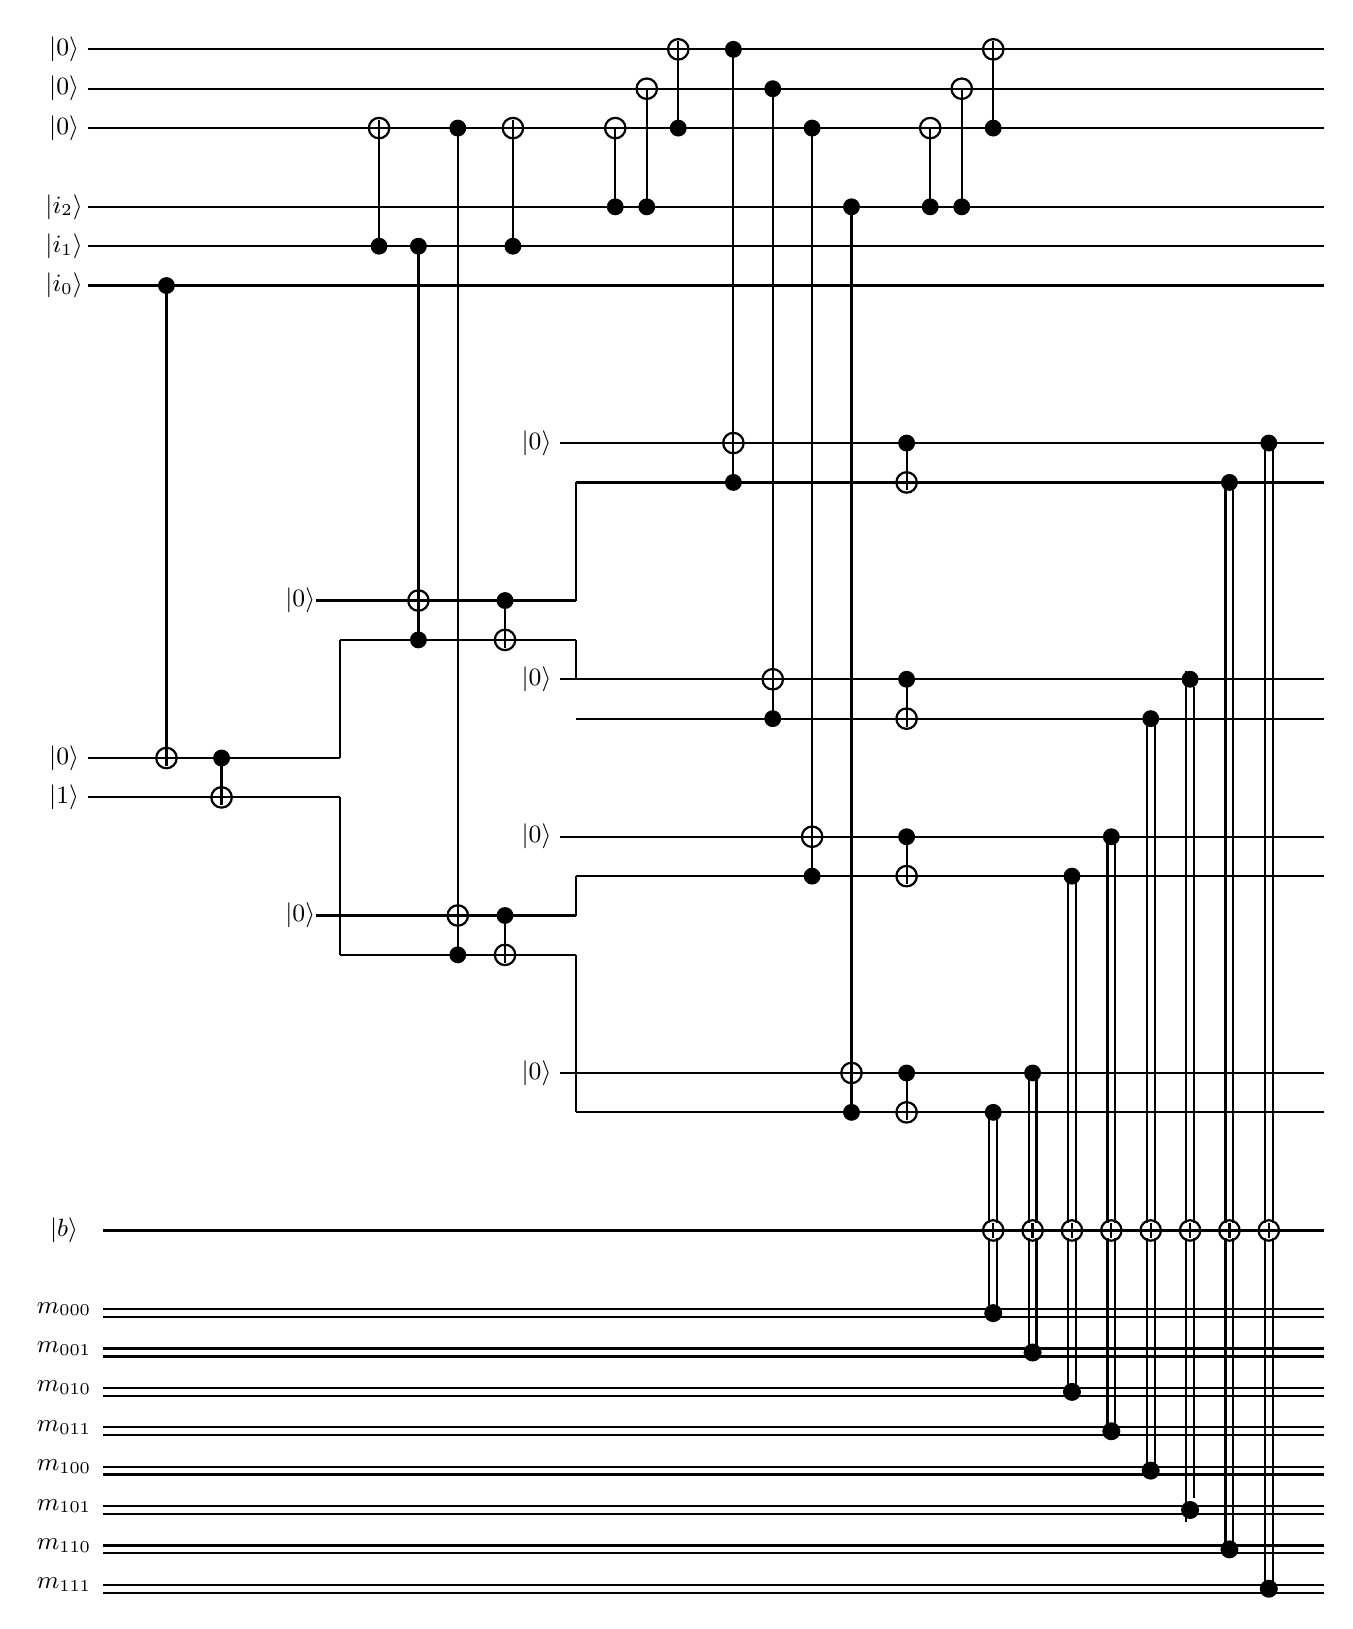
\begin{tikzpicture}
    % address register
    \draw (0, 0) node{\small $\ket{i_0}$};
    \draw (0, 0.5) node{\small $\ket{i_1}$};
    \draw (0, 1) node{\small $\ket{i_2}$};

    % memory register
    \draw (0, -13) node{\small $m_{000}$};
    \draw (0, -13.5) node{\small $m_{001}$};
    \draw (0, -14) node{\small $m_{010}$};
    \draw (0, -14.5) node{\small $m_{011}$};
    \draw (0, -15) node{\small $m_{100}$};
    \draw (0, -15.5) node{\small $m_{101}$};
    \draw (0, -16) node{\small $m_{110}$};
    \draw (0, -16.5) node{\small $m_{111}$};

    % ancilla qubits register
    \draw (0, 2) node{\small $\ket{0}$};
    \draw (0, 2.5) node{\small $\ket{0}$};
    \draw (0, 3) node{\small $\ket{0}$};
    

    % target register 
    \draw (0, -12) node{\small $\ket{b}$};

    % horizontal line ancilla register
    \draw [-] [thick] (0+0.3, 2) to (16, 2);
    \draw [-] [thick] (0+0.3, 2.5) to (16, 2.5);
    \draw [-] [thick] (0+0.3, 3) to (16, 3);

    % horizontal lines address register
    \draw [-] [thick] (0+0.3, 0) to (16, 0);
    \draw [-] [thick] (0+0.3, 0.5) to (16, 0.5);
    \draw [-] [thick] (0+0.3, 1) to (16, 1);

    % horizontali lines memory and target 
    \draw [-] [thick] (0+0.5, -13-0.1) to (16, -13-0.1);
  \draw [-] [thick] (0+0.5, -13.5-0.1) to (16, -13.5-0.1);
  \draw [-] [thick] (0+0.5, -14-0.1) to (16, -14-0.1);
   \draw [-] [thick] (0+0.5, -14.5-0.1) to (16, -14.5-0.1);
   \draw [-] [thick] (0+0.5, -15-0.1) to (16, -15-0.1);
   \draw [-] [thick] (0+0.5, -15.5-0.1) to (16, -15.5-0.1);
   \draw [-] [thick] (0+0.5, -16.5-0.1) to (16, -16.5-0.1);
   \draw [-] [thick] (0+0.5, -16-0.1) to (16, -16-0.1);
  \draw [-] [thick] (0+0.5, -12) to (16, -12);

    % double lines for classical memory register
      \draw [-] [thick] (0+0.5, -13) to (16, -13);
  \draw [-] [thick] (0+0.5, -13.5) to (16, -13.5);
  \draw [-] [thick] (0+0.5, -14) to (16, -14);
   \draw [-] [thick] (0+0.5, -14.5) to (16, -14.5);
   \draw [-] [thick] (0+0.5, -15) to (16, -15);
   \draw [-] [thick] (0+0.5, -15.5) to (16, -15.5);
   \draw [-] [thick] (0+0.5, -16.5) to (16, -16.5);
   \draw [-] [thick] (0+0.5, -16) to (16, -16);
 


    % ANCILLA REGISTERS
    % central ancilla register
    \draw (0, -6) node{\small $\ket{0}$};
    \draw (0, -6.5) node{\small $\ket{1}$};

    % above and below angilla register pt 2
    \draw (3, -4) node{\small $\ket{0}$};
    %\draw (3, -4.5) node{\small $\ket{1}$};

    \draw (3, -8) node{\small $\ket{0}$};
    %\draw (3, -8.5) node{\small $\ket{1}$};


    % above and below kets pt 3
    \draw (6, -2) node{\small $\ket{0}$};
    %\draw (6, -2.5) node{\small $\ket{1}$};

    \draw (6, -10) node{\small $\ket{0}$};
    %\draw (6, -10.5) node{\small $\ket{1}$};

    \draw (6, -5) node{\small $\ket{0}$};
    %\draw (6, -5.5) node{\small $\ket{1}$};

    \draw (6, -7) node{\small $\ket{0}$};
    %\draw (6, -7.5) node{\small $\ket{1}$};



    % horizontal lines 2nd level of ancillas
    \draw [-] [thick] (0+0.3, -6) to (3+0.5, -6);   % 0 
    \draw [-] [thick] (0+0.3, -6.5) to (3+0.5, -6.5);  % 1


    % % horizontal lines pt 2
    \draw [-] [thick] (3+0.5, -4.5) to (3+3.5, -4.5);   % 1
    \draw [-] [thick] (3+0.5, -8.5) to (3+3.5, -8.5);   % 1
    
    \draw [-] [thick] (3+0.2, -4) to (3+3.5, -4);   % 0
    \draw [-] [thick] (3+0.2, -8) to (3+3.5, -8);   % 0


    % % horizontal lines pt 3 
    \draw [-] [thick] (6+0.5-0.2, -2) to (16, -2);   % 0
    \draw [-] [thick] (6+0.5, -2.5) to (16, -2.5);   % 1

    \draw [-] [thick] (6+0.5-0.2, -5) to (16, -5);   % 0
    \draw [-] [thick] (6+0.5, -5.5) to (16, -5.5);   % 1

    \draw [-] [thick] (6+0.5-0.2, -7) to (16, -7);   % 0
    \draw [-] [thick] (6+0.5, -7.5) to (16, -7.5);   % 1

    \draw [-] [thick] (6+0.5-0.2, -10) to (16, -10);   % 0
    \draw [-] [thick] (6+0.5, -10.5) to (16, -10.5);   % 1

    
    % vertical lines (central to external)
    \draw [-] [thick] (3+0.5, -6) to (3+0.5, -4.5); % 0 -> 1
    \draw [-] [thick] (3+0.5, -6.5) to (3+0.5, -8.5); 
    \draw [-] [thick] (6+0.5, -4) to (6+0.5, -2.5);
    \draw [-] [thick] (6+0.5, -4.5) to (6+0.5, -5);
    \draw [-] [thick] (6+0.5, -8.5) to (6+0.5, -10.5);   % 4th
    \draw [-] [thick] (6+0.5, -8) to (6+0.5, -7.5);



     % CNOTS first layer
     \draw[fill=black] (0+0.3+1, 0) circle [radius=0.1];
     \draw (0+0.3+1, -6) [thick] circle (0.13);
     \draw [-] [thick] (0+0.3+1, 0) to (0+0.3+1, -6);
     \draw [-] [thick] (0+0.3+1, -6-0.1) to (0+0.3+1, -6+0.1);

    \draw[fill=black] (2, -6) circle [radius=0.1];
     \draw (2, -6.5) [thick] circle (0.13);
     \draw [-] [thick] (2, -6) to (2, -6.5);
     \draw [-] [thick] (2, -6.5+0.1) to (2, -6.5-0.1);

    % COPY SECOND REGISTER
    \draw[fill=black] (3+1, 0.5) circle [radius=0.1];
   \draw (3+1, 2) [thick] circle (0.13);
   \draw [-] [thick] (3+1, 0.5) to (3+1, 2.1);

    
    % CCNOT of second layer
   \draw[fill=black] (3+0.5+1, 0.5) circle [radius=0.1];
   \draw (3+0.5+1, -4) [thick] circle (0.13);
   \draw [-] [thick] (3+0.5+1, 0.5) to (3+0.5+1, -4);
   \draw [-] [thick] (3+0.5+1, -4.5) to (3+0.5+1, -4);
    \draw[fill=black] (3+0.5+1, -4.5) circle [radius=0.1];

    \draw[fill=black] (3+0.3+1+0.5+0.2, 2) circle [radius=0.1];
    \draw (3+0.3+1+0.5+0.2, -8) [thick] circle (0.13);
    \draw [-] [thick] (3+0.3+1+0.5+0.2, 2) to (3+0.3+1+0.5+0.2, -8.5);
    \draw [-] [thick] (3+0.3+1+0.5+0.2, -4.5) to (3+0.3+1+0.5+0.2, -4);
    \draw[fill=black] (3+0.3+1+0.5+0.2, -8.5) circle [radius=0.1];


    % last two CNOTs of second layer
    \draw[fill=black] (5.6, -4) circle [radius=0.1];
     \draw (5.6, -4.5) [thick] circle (0.13);
     \draw [-] [thick] (5.6, -4) to (5.6, -4.5);
     \draw [-] [thick] (5.6, -4.5+0.1) to (5.6, -4.5-0.1);

    \draw[fill=black] (5.6, -8) circle [radius=0.1];
     \draw (5.6, -8.5) [thick] circle (0.13);
     \draw [-] [thick] (5.6, -8) to (5.6, -8.5);
     \draw [-] [thick] (5.6, -8.5+0.1) to (5.6, -8.5-0.1);

    % add cnot that uncomputes the first copy
    \draw[fill=black] (3+2.7, 0.5) circle [radius=0.1];
   \draw (3+2.7, 2) [thick] circle (0.13);
   \draw [-] [thick] (3+2.7, 0.5) to (3+2.7, 2.1);


    % COPY INDEX
    \draw[fill=black] (7, 1) circle [radius=0.1];
    \draw (7, 2) [thick] circle (0.13);
     \draw [-] [thick] (7, 2) to (7, 1);

    \draw[fill=black] (7.4, 1) circle [radius=0.1];
    \draw (7.4, 2.5) [thick] circle (0.13);
     \draw [-] [thick] (7.4, 2.5) to (7.4, 1);

    \draw[fill=black] (7.8, 2) circle [radius=0.1];
    \draw (7.8, 3) [thick] circle (0.13);
    \draw [-] [thick] (7.8, 3.1) to (7.8, 2);


     % box to say that we copy
     % \draw [-] [dotted,thick]  (6.5, 3.2) to (8.2, 3.2);
     % \draw [-] [dotted,thick]  (8.2, 0.5) to (8.2, 3.2);
     % \draw [-] [dotted,thick]  (8.2, 0.4) to (6.5, 0.4);
     % \draw [-] [dotted]  (6.5, 0.4) to (6.5, 3.2);
     

    % last CCNOT on (copied) index register 
    \draw[fill=black] (8.5, 3) circle [radius=0.1];
    \draw[fill=black] (8.5, -2.5) circle [radius=0.1];
    \draw (8.5, -2) [thick] circle (0.13);
     \draw [-] [thick] (8.5, -2.5) to (8.5, 3);



    \draw[fill=black] (9, 2.5) circle [radius=0.1];
    \draw[fill=black] (9, -5.5) circle [radius=0.1];
    \draw (9, -5) [thick] circle (0.13);
     \draw [-] [thick] (9, -5.5) to (9, 2.5);


    \draw[fill=black] (9.5, 2) circle [radius=0.1];
    \draw[fill=black] (9.5, -7.5) circle [radius=0.1];
    \draw (9.5, -7) [thick] circle (0.13);
     \draw [-] [thick] (9.5, -7.5) to (9.5, 2);

     
    \draw[fill=black] (10, 1) circle [radius=0.1];
    \draw[fill=black] (10, -10.5) circle [radius=0.1];
    \draw (10, -10) [thick] circle (0.13);
     \draw [-] [thick] (10, -10.5) to (10, 1);


     % last layer of cnots
    % \draw[fill=black] (8.5, -2) circle [radius=0.1];
    \draw[fill=black] (9+1.7, -2) circle [radius=0.1];
    \draw (9+1.7, -2.5) [thick] circle (0.13);
    \draw [-] [thick] (9+1.7, -2.5-0.1) to (9+1.7, -2);
     
    \draw[fill=black] (9+1.7, -5) circle [radius=0.1];
    \draw (9+1.7, -5.5) [thick] circle (0.13);
    \draw [-] [thick] (9+1.7, -5.5-0.1) to (9+1.7, -5);


    \draw[fill=black] (9+1.7, -7) circle [radius=0.1];
    \draw (9+1.7, -7.5) [thick] circle (0.13);
    \draw [-] [thick] (9+1.7, -7.5-0.1) to (9+1.7, -7);

    \draw[fill=black] (9+1.7, -10) circle [radius=0.1];
    \draw (9+1.7, -10.5) [thick] circle (0.13);
    \draw [-] [thick] (9+1.7, -10.5-0.1) to (9+1.7, -10);

    % writing in memory (OK)
    % \draw[fill=black] (9.5+2.3, -10.5) circle [radius=0.1];
    % \draw[fill=black] (9.5+2.3, -13-0.05) [thick] circle (0.1);
    % \draw (9.5+2.3, -12) [thick] circle (0.13);
    % \draw [-] [thick] (9.5+2.3, -10.5) to (9.5+2.3, -13-0.1);

    % \draw[fill=black] (10+2.3, -10) circle [radius=0.1];
    % \draw[fill=black] (10+2.3, -13.5-0.05) [thick] circle (0.1);
    % \draw (10+2.3, -12) [thick] circle (0.13);
    % \draw [-] [thick] (10+2.3, -10) to (10+2.3, -13.5-0.1);

    % \draw[fill=black] (10.5+2.3, -7.5) circle [radius=0.1];
    % \draw[fill=black] (10.5+2.3, -14-0.05) [thick] circle (0.1);
    % \draw (10.5+2.3, -12) [thick] circle (0.13);
    % \draw [-] [thick] (10.5+2.3, -7.5) to (10.5+2.3, -14-0.1);

    % \draw[fill=black] (11+2.3, -7) circle [radius=0.1];
    % \draw[fill=black] (11+2.3, -14.5-0.05) [thick] circle (0.1);
    % \draw (11+2.3, -12) [thick] circle (0.13);
    % \draw [-] [thick] (11+2.3, -7) to (11+2.3, -14.5-0.1);


    % \draw[fill=black] (11.5+2.3, -5.5) circle [radius=0.1];
    % \draw[fill=black] (11.5+2.3, -15-0.05) [thick] circle (0.1);
    % \draw (11.5+2.3, -12) [thick] circle (0.13);
    % \draw [-] [thick] (11.5+2.3, -5.5) to (11.5+2.3, -15-0.1);

    % \draw[fill=black] (12+2.3, -5) circle [radius=0.1];
    % \draw[fill=black] (12+2.3, -15.5-0.05) [thick] circle (0.1);
    % \draw (12+2.3, -12) [thick] circle (0.13);
    % \draw [-] [thick] (12+2.3, -5) to (12+2.3, -15.5-0.1);


    % \draw[fill=black] (12.5+2.3, -2.5) circle [radius=0.1];
    % \draw[fill=black] (12.5+2.3, -16-0.05) [thick] circle (0.1);
    % \draw (12.5+2.3, -12) [thick] circle (0.13);
    % \draw [-] [thick] (12.5+2.3, -2.5) to (12.5+2.3, -16-0.1);

    % \draw[fill=black] (13+2.3, -2) circle [radius=0.1];
    % \draw[fill=black] (13+2.3, -16.5-0.05) [thick] circle (0.1);
    % \draw (13+2.3, -12) [thick] circle (0.13);
    % \draw [-] [thick] (13+2.3, -2) to (13+2.3, -16.5-0.1);

    \draw[fill=black] (9.5+2.3, -10.5) circle [radius=0.1];
    \draw[fill=black] (9.5+2.3, -13-0.05) [thick] circle (0.1);
    \draw (9.5+2.3, -12) [thick] circle (0.13);
    \draw [-] [thick] (9.5+2.3-0.05, -10.5) to (9.5+2.3-0.05, -12+0.1);
    \draw [-] [thick] (9.5+2.3-0.05, -12-0.1) to (9.5+2.3-0.05, -13-0.1);
    \draw [-] [thick] (9.5+2.3+0.05, -10.5) to (9.5+2.3+0.05, -12+0.1);
    \draw [-] [thick] (9.5+2.3+0.05, -12-0.1) to (9.5+2.3+0.05, -13-0.1);


    \draw[fill=black] (10+2.3, -10) circle [radius=0.1];
    \draw[fill=black] (10+2.3, -13.5-0.05) [thick] circle (0.1);
    \draw (10+2.3, -12) [thick] circle (0.13);
    \draw [-] [thick] (10+2.3-0.05, -10) to (10+2.3-0.05, -12+0.1);
    \draw [-] [thick] (10+2.3-0.05, -12-0.1) to (10+2.3-0.05, -13.5-0.1);
    \draw [-] [thick] (10+2.3+0.05, -10) to (10+2.3+0.05, -12+0.1);
    \draw [-] [thick] (10+2.3+0.05, -12-0.1) to (10+2.3+0.05, -13.5-0.1);



    \draw[fill=black] (10.5+2.3, -7.5) circle [radius=0.1];
    \draw[fill=black] (10.5+2.3, -14-0.05) [thick] circle (0.1);
    \draw (10.5+2.3, -12) [thick] circle (0.13);
    \draw [-] [thick] (10.5+2.3-0.05, -7.5) to (10.5+2.3-0.05, -12+0.1);
    \draw [-] [thick] (10.5+2.3-0.05, -12-0.1) to (10.5+2.3-0.05, -14-0.1);
    \draw [-] [thick] (10.5+2.3+0.05, -7.5) to (10.5+2.3+0.05, -12+0.1);
    \draw [-] [thick] (10.5+2.3+0.05, -12-0.1) to (10.5+2.3+0.05, -14-0.1);



    \draw[fill=black] (11+2.3, -7) circle [radius=0.1];
    \draw[fill=black] (11+2.3, -14.5-0.05) [thick] circle (0.1);
    \draw (11+2.3, -12) [thick] circle (0.13);
    \draw [-] [thick] (11+2.3-0.05, -7) to (11+2.3-0.05, -12+0.1);
    \draw [-] [thick] (11+2.3-0.05, -12-0.1) to (11+2.3-0.05, -14.5-0.1);
    \draw [-] [thick] (11+2.3+0.05, -7) to (11+2.3+0.05, -12+0.1);
    \draw [-] [thick] (11+2.3+0.05, -12-0.1) to (11+2.3+0.05, -14.5-0.1);


    \draw[fill=black] (11.5+2.3, -5.5) circle [radius=0.1];
    \draw[fill=black] (11.5+2.3, -15-0.05) [thick] circle (0.1);
    \draw (11.5+2.3, -12) [thick] circle (0.13);
    \draw [-] [thick] (11.5+2.3-0.05, -5.5) to (11.5+2.3-0.05, -12+0.1);
    \draw [-] [thick] (11.5+2.3-0.05, -12-0.1) to (11.5+2.3-0.05, -15-0.1);
    \draw [-] [thick] (11.5+2.3+0.05, -5.5) to (11.5+2.3+0.05, -12+0.1);
    \draw [-] [thick] (11.5+2.3+0.05, -12-0.1) to (11.5+2.3+0.05, -15-0.1);


    \draw[fill=black] (12+2.3, -5) circle [radius=0.1];
    \draw[fill=black] (12+2.3, -15.5-0.05) [thick] circle (0.1);
    \draw (12+2.3, -12) [thick] circle (0.13);
    \draw [-] [thick] (12+2.3-0.05, -5+0.1) to (12+2.3-0.05, -12-0.1+0.2);
    \draw [-] [thick] (12+2.3-0.05, -12-0.1) to (12+2.3-0.05, -15.5-0.1-0.1);
    \draw [-] [thick] (12+2.3+0.05, -12-0.1) to (12+2.3+0.05, -15.5-0.1+0.2);
    \draw [-] [thick] (12+2.3+0.05, -12+0.1) to (12+2.3+0.05, -5-0.1);
    


    \draw[fill=black] (12.5+2.3, -2.5) circle [radius=0.1];
    \draw[fill=black] (12.5+2.3, -16-0.05) [thick] circle (0.1);
    \draw (12.5+2.3, -12) [thick] circle (0.13);
    \draw [-] [thick] (12.5+2.3-0.05, -2.5) to (12.5+2.3-0.05, -12+0.1);
    \draw [-] [thick] (12.5+2.3-0.05, -12-0.1) to (12.5+2.3-0.05, -16);
    \draw [-] [thick] (12.5+2.3+0.05, -2.5) to (12.5+2.3+0.05, -12+0.1);
    \draw [-] [thick] (12.5+2.3+0.05, -12-0.1) to (12.5+2.3+0.05, -16);
    
    % \draw [-] [thick] (12.5+2.3, -2.5) to (12.5+2.3, -16-0.1);
    % \draw [-] [thick] (12.5+2.3, -2.5) to (12.5+2.3, -16-0.1);
    % \draw [-] [thick] (12.5+2.3, -2.5) to (12.5+2.3, -16-0.1);





    \draw[fill=black] (13+2.3, -2) circle [radius=0.1];
    \draw[fill=black] (13+2.3, -16.5-0.05) [thick] circle (0.1);
    \draw (13+2.3, -12) [thick] circle (0.13);
    \draw [-] [thick] (13+2.3-0.05, -2) to (13+2.3-0.05, -12+0.1);
    \draw [-] [thick] (13+2.3-0.05, -12-0.1) to (13+2.3-0.05, -16.5-0.1);
    \draw [-] [thick] (13+2.3+0.05, -2) to (13+2.3+0.05, -12+0.1);
    \draw [-] [thick] (13+2.3+0.05, -12-0.1) to (13+2.3+0.05, -16.5-0.1);


% NOT vertical line
 \draw [-] [thick] (13+2.3, -12+0.1) to (13+2.3, -12-0.1);
 \draw [-] [thick] (12.5+2.3, -12+0.1) to (12.5+2.3, -12-0.1);
\draw [-] [thick] (12+2.3, -12+0.1) to (12+2.3, -12-0.1);
\draw [-] [thick] (11.5+2.3, -12+0.1) to (11.5+2.3, -12-0.1);
\draw [-] [thick] (11+2.3, -12+0.1) to (11+2.3, -12-0.1);
\draw [-] [thick] (10.5+2.3, -12+0.1) to (10.5+2.3, -12-0.1);
\draw [-] [thick] (10+2.3, -12+0.1) to (10+2.3, -12-0.1);
\draw [-] [thick] (9.5+2.3, -12+0.1) to (9.5+2.3, -12-0.1);
%

    % \draw [-] [thick] (13+2.3, -12) to (13+2.3, -16.5-0.1);
    % \draw [-] [thick] (13+2.3, -12) to (13+2.3, -16.5-0.1);
    % \draw [-] [thick] (13+2.3, -12) to (13+2.3, -16.5-0.1);
    % \draw [-] [thick] (13+2.3, -12) to (13+2.3, -16.5-0.1);
    % \draw [-] [thick] (13+2.3, -12) to (13+2.3, -16.5-0.1);
    % \draw [-] [thick] (13+2.3, -12) to (13+2.3, -16.5-0.1);
    % \draw [-] [thick] (13+2.3, -12) to (13+2.3, -16.5-0.1);





     
    % TODO undo the last copy
    \draw[fill=black] (11, 1) circle [radius=0.1];
    \draw (11, 2) [thick] circle (0.13);
     \draw [-] [thick] (11, 2) to (11, 1);

    \draw[fill=black] (11.4, 1) circle [radius=0.1];
    \draw (11.4, 2.5) [thick] circle (0.13);
     \draw [-] [thick] (11.4, 2.5) to (11.4, 1);

    \draw[fill=black] (11.8, 2) circle [radius=0.1];
    \draw (11.8, 3) [thick] circle (0.13);
    \draw [-] [thick] (11.8, 3.1) to (11.8, 2);

\end{tikzpicture}




\end{document}